% This workshop aims to surface future NIME leaders. We will introduce these people to the practicalities of organising NIME and in-between NIME activities, and co-design future NIME initiatives and conference plans. We interpret NIME leaders broadly and inclusively to mean anybody who is ready (now or in the future) to contribute to our community beyond conference submissions and reviews. This could mean metareviewing, leading initiatives, moderating the forum, volunteering as a future conference chair, aspiring to host a future NIME, supporting or organising committees, running for election to the board, or imagining new NIME activities that nobody has thought of before! We are looking for future leaders with energy and enthusiasm at all career stages and from all backgrounds. Workshop facilitators will include former NIME chairs and members of the NIME board. Be careful about walking in the door---you will very likely walk out with a new job (and also a lot of new friends)!

% - This workshop will require a classroom or similar space, ideally with multiple tables for small group discussions and co-design activities.
% - A projector and screen will be required.

% up to the capacity of the space - 40 participants would be fine.

\documentclass[acmsmall]{nimeart}

\setcopyright{cc}
\copyrightyear{2026}
\acmYear{2026}
\acmDOI{}

\acmConference[NIME '26]{International Conference on New Interfaces for Musical Expression}{June 23--26,
  2026}{London, UK}

\settopmatter{printacmref=false}

\acmISBN{}

\begin{document}

\title{Future NIME Leaders Workshop}

\author{Charles Patrick Martin}
\affiliation{%
  \institution{Australian National University}
  \city{Canberra}
  \country{Australia}
}

\author{Stefano Fasciani}
\affiliation{%
  \institution{University of Oslo}
  \city{Oslo}
  \country{Norway}
}

\author{Juan Martinez Avila}
\affiliation{%
  \institution{University of Nottingham}
  \city{Nottingham}
  \country{United Kingdom}
}

\author{Fabio Morreale}
\affiliation{%
  \institution{Sony AI}
  \city{Barcelona}
  \country{Spain}
}

\author{Andrew McPherson}
\affiliation{%
  \institution{Imperial College London}
  \city{London}
  \country{United Kingdom}
}

\author{Courtney N. Reed}
\affiliation{%
  \institution{Loughborough University London}
  \city{London}
  \country{United Kingdom}
}

\author{Pia van Gelder}
\affiliation{%
  \institution{Australian National University}
  \city{Canberra}
  \country{Australia}
}

\author{Yichen Wang}
\affiliation{%
  \institution{Australian National University}
  \city{Canberra}
  \country{Australia}
}

\author{Doga Cavdir}
% \email{dogc@itu.dk}
% \orcid{0000-0003-0169-2945}
\affiliation{%
  \institution{IT University of Copenhagen}
  \city{Copenhagen}
  \state{}
  \country{Denmark}
}

\renewcommand{\shortauthors}{Martin et al.}

\begin{abstract}
This workshop aims to surface future NIME leaders. We will introduce these people to the practicalities of organising NIME and in-between NIME activities, and co-design future NIME initiatives and conference plans.
We interpret NIME leaders broadly and inclusively to mean anybody who is ready (now or in the future) to contribute to our community beyond conference submissions and reviews. Leadership contributions could entail becoming a metareviewer, leading initiatives, being active on the NIME forum, volunteering as a future conference chair, aspiring to host a future NIME, supporting or organising committees, running for election to the board, or imagining new NIME activities that nobody has thought of before! 
We are looking for future leaders with energy and enthusiasm at all career stages and from all backgrounds. 
Workshop facilitators will include former NIME chairs and members of the NIME board.
Be careful about walking in the door---you will very likely walk out with a new job (and also a lot of new friends)!
\end{abstract}

\keywords{leadership, conference, organising, service}

\maketitle

\section{Motivation} 

NIME is a volunteer community with many ways to contribute and many opportunities for leadership. However, as in many communities, help is always needed, particularly to meet our goals of broadening participation and becoming more inclusive. The motivation of this workshop is to surface future NIME leaders. That is, people who are ready (now or in the future) to contribute to our community beyond conference submissions and reviews.
This is not just about becoming a general chair but about acknowledging the many roles in NIME and the many ways leadership can be displayed. We seek to break down some of the systemic barriers that prevent community members from knowing that their help is welcome and, often, very much needed.
We invite people who have energy and enthusiasm at all career stages and backgrounds to participate. The only limitation is that you may end up with a new job at the end of the workshop!

\section{Workshop Structure}

The workshop would run for 3 hours but the plan is flexible so that the length fits with the workshop chairs' plans.

\subsection{Introduction to the NIME organisation}

This section will introduce participants to the organisation behind the NIME conference as well as the different roles that typically participate in the conference organisation. We will cover (at least):
\begin{itemize}
    \item the NIME board
    \item NIME committees
    \item NIME forum and mailing list
    \item typical conference chairs
    \item meta-reviewers and reviewers
    \item other volunteer and support roles
\end{itemize}
The goal of this session is not just information delivery. By discussing a very broad range of roles, we will challenge participants to reflect on where they could see themselves now and in future. The organisational discussion will be a catalyst for learning from participants about their background and the different skills and experience they could bring to NIME.

\begin{figure}
    \centering
    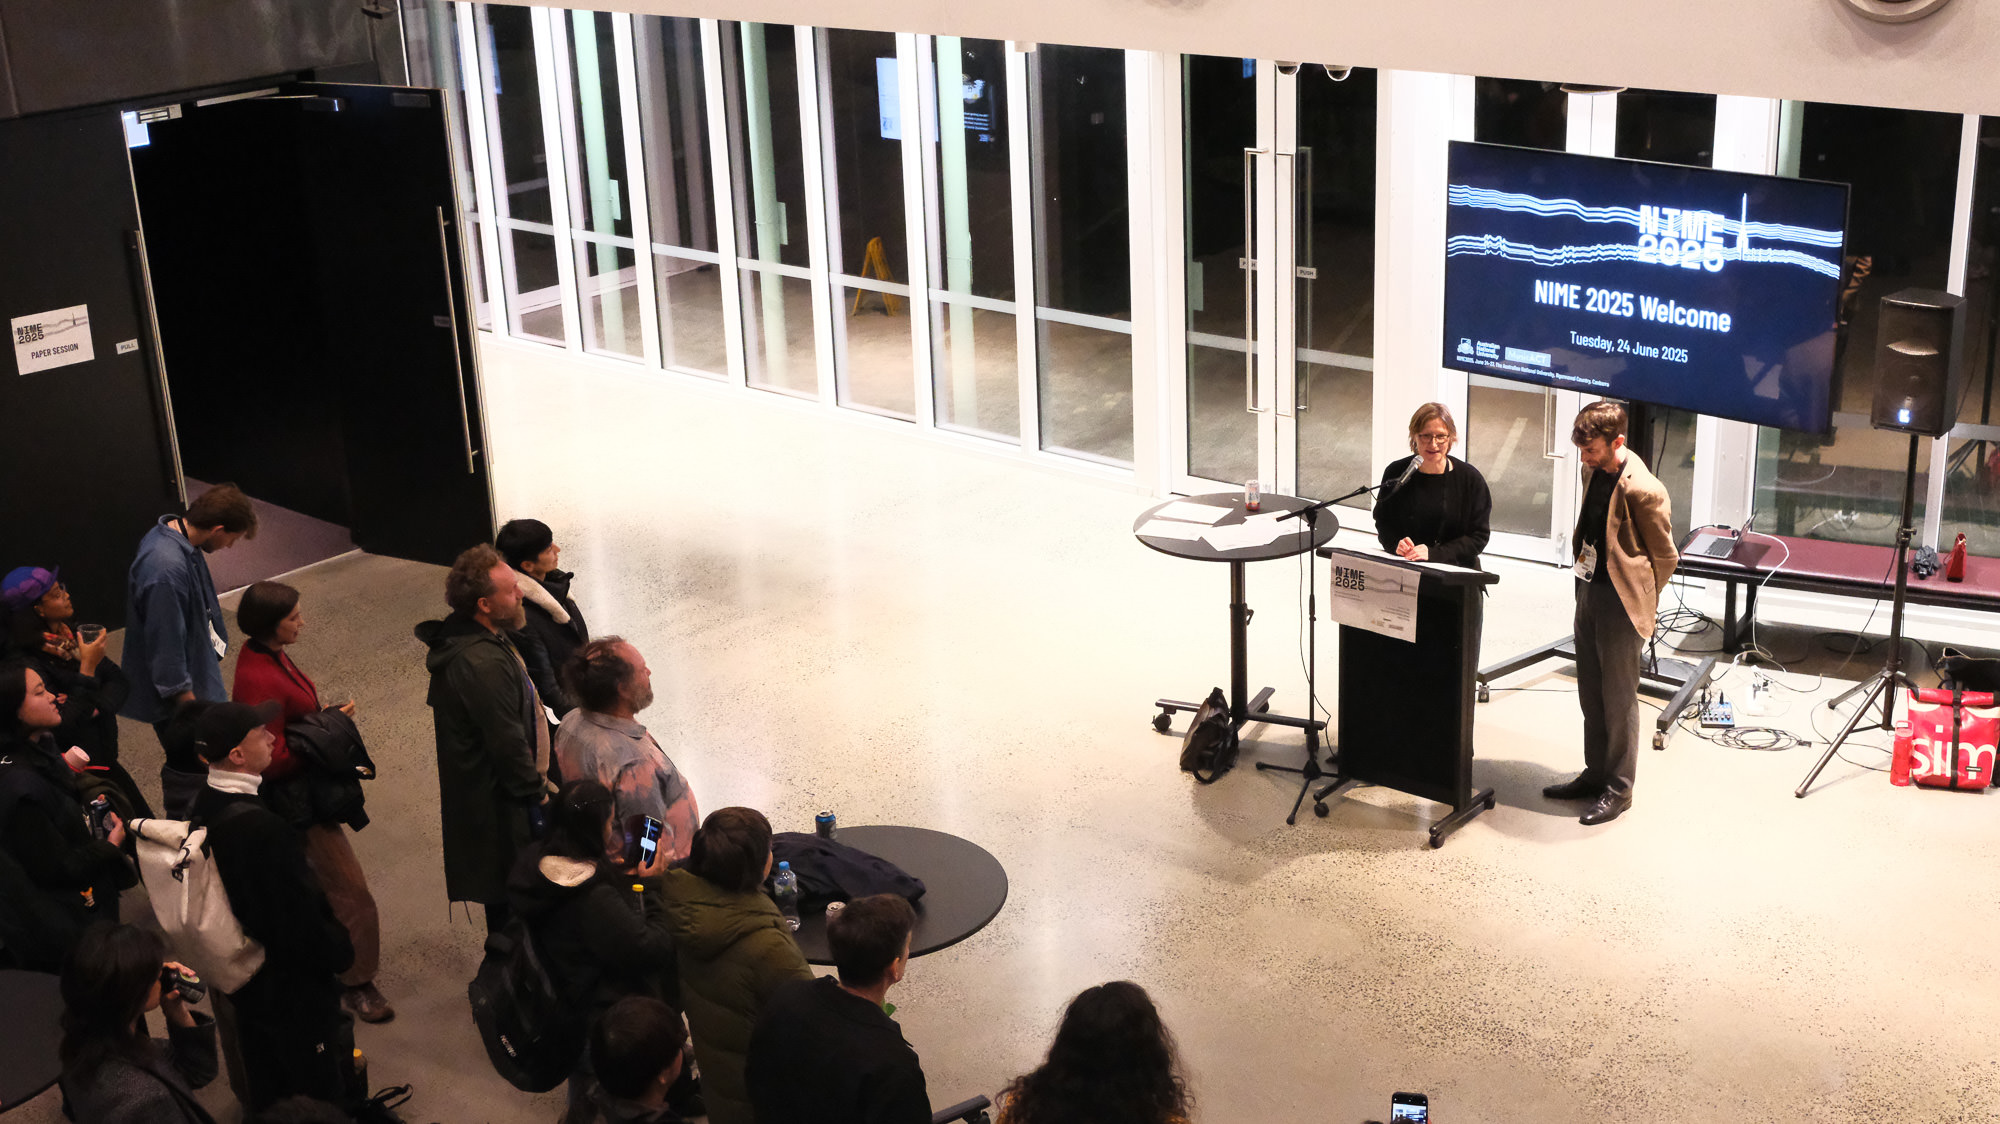
\includegraphics[width=0.75\linewidth]{images/nime-leaders-workshop-2000.jpg}
    \caption{Pia and Charles at NIME2025. This could be you!}
    \label{fig:nime-leadership-image}
\end{figure}

\subsection{So, you want to propose a NIME...}

This session starts with the following provocation:
\begin{quote}
  \emph{NIME president, Fabio Morreale, just called and YOU are running next year's NIME. You're up for it, but we need your proposal by tomorrow! What do you do?}
\end{quote}
In this session we will challenge participants to plan a NIME in an hour (seriously!)
We will introduce the (new) NIME hosting proposal template\footnote{\url{https://github.com/NIME-conference/nime-hosting-proposal-template/}}, and NIME cookbook\footnote{\url{https://github.com/NIME-conference/NIME-cookbook}}.

While it might be fun to plan a \emph{dream conference} where money is no object, we really want participants to look at the resources they do have and work out what kind of NIME they could put together if they really had to do it.
The broader goal is to learn what future conference organisers could bring to our community and what they might need to really run a conference. We hope that among our participants will be people who become future NIME hosts!

Our session will explore misconceptions about conference hosting, and volunteer roles in conference organisation in terms of what they involve, the resources that are already available, and the kind of support and infrastructure that is present behind the scenes.

While we will embrace experimental and untried approaches to NIME in this session we will balance the "nice-to-haves" of hosting with the other side of the realities that previous organisers have faced in terms of finances,  bureaucracy, spaces, and resources.

\subsection{Co-designing unknown NIME initiatives}

This session seeks to speculate on the missing parts of our community. 
We will use design prompts and ideation exercises to generate and critique new kinds of activities, roles, groups, or resources that are currently missing from NIME.
These (so far) unknown activities could become \emph{core} parts of NIME in future, so it is critical to continually generate, articulate, and demonstrate new initiatives.

We will reflect again on Dr Clare Cooper's challenge to NIME in the 2025 keynote\footnote{\url{https://nime2025.org/sessions/keynote-1.html}}:
\begin{itemize}
    \item What shall we gleefully abandon?
    \item What shall we boldly launch?
    \item What shall we lovingly maintain?
\end{itemize}
Again, while we will be open ended in ideation, the second half of this session will challenge participants to choose which ideas can and should be made real, and to plan how. 

At the end of this session, some future NIME leaders will have an idea, a mandate for action, and will be ready to \emph{boldly launch} into their new role in our community!

\section{Organisers}

% Organisers: Include Workshop organiser(s) with short bios.

\begin{description}
    
\item[Charles Martin] was a general chair of NIME2025, was elected to the NIME board in 2024 and has been a NIME author since 2010.
Charles aspires to strengthen NIME's impact and resilience by involving a broader group of future leaders and creating new opportunities for activity outside of the yearly conference.
Charles is a computer science academic at the Australian National University. \url{https://charlesmartin.au}

\item[Stefano Fasciani] was elected to the NIME board as Proceedings Officer in 2024 and has been a NIME author since 2012.
Stefano aims to involve members of the community in improving how NIME’s material and information are archived and preserved throughout the years, ensuring longevity, sustainability, and visibility. He also aims to reorganise and recover older NIME material that was archived according to previous practices. In addition, he seeks to foster new ways for members of the NIME community to collaborate more actively beyond the short meetings held at the yearly conference.
Stefano is a music technology academic at the University of Oslo. \url{https://stefanofasciani.com}

\item[Juan Martinez Avila] is an assistant professor in computer science at the University of Nottingham, and a human-computer interaction researcher, specialised in embodied interaction and music interaction. He became part of the NIME Board in 2024, joining as Chair of Committees. His role is to liaise and coordinate with the leads of the various NIME committees, such as, Diversity, Ethics, Ecology and other initiatives like WiNIME (Women in NIME) and the LATAM (Latin American) NIME Network. He first attended NIME in 2018 and has been involved in NIME volunteering since 2019, either as a reviewer and meta-reviewer, diversity officer (2021--2024), LATAM NIME Network founder and member at large (2021--Now).
\url{https://www.avila.jp.net/}

\item[Fabio Morreale] is the current president of the NIME board, was a general chair of NIME2022, and has been attending NIME since 2012. From 2020 to 2022 he was the Chair of the NIME Ethics committee and led the development of the first version of the Code of Ethics. Now a Staff Research Scientist at Sony AI, Fabio works in the intersection of NIME, AI, Ethics, and Philosophy of Technology. Prior to that, he was a Senior Lecturer at the University of Auckland in New Zealand and a postdoc at Queen Mary University of London in the Augmented Instruments Lab.  \url{https://fabio.kiwi}

\item[Andrew McPherson] is Professor of Design Engineering and Music at Imperial College London, where he leads the Augmented Instruments Laboratory. A composer, viola player, electronic engineer and HCI researcher by training, he has been attending NIME since 2010 and has served as paper chair twice (2016, 2022); he is a general co-chair of NIME 2026. He has also served on the NIME board as Continuity Officer. \url{https://andrewmcpherson.org}

\item[Courtney N. Reed] is a vocalist and Lecturer/Assistant Professor in Digital Technologies and Creative Futures at Loughborough University London. She specialises in HCI and design for vocal bodies. Courtney first attended NIME in 2020 and has since served as paper chair (2024), Diversity Committee co-lead (2024-), and general co-chair for NIME 2026. She was also on the NIME Board as Member-at-Large (2024-2026) and is the Chair 2026 representative. She is active in building formal and informal networks for early career researchers (ECRs) across NIME and adjacent HCI communities. She previously organised the annual Women in Music Information Retrieval (WiMIR) Workshop (2021-2022). \url{https://www.courtneynreed.com/}

\item[Pia van Gelder] is an electronic artist, researcher and historian. Her art practice and scholarship
investigate historical and contemporary conceptions of energy and how these shape our relationship
with technology, bodies and our environment. Her recent scholarship has concentrated on the influence
of esotericism on electronic instruments of the 20th century. She is an academic in the College of Arts and
Social Sciences at the Australian National University. Pia was a general chair of NIME2025 and has a track record curating events and artist run initiatives including Serial Space (Sydney), one of the venues for NIME2010. \url{https://piavangelder.com/}

\item[Yichen Wang] is a postdoctoral researcher working on musical interaction design in augmented reality and co-creative systems in HCI at CRIStAL - Universit{é} de Lille. Yichen has been attending the annual NIME conference since 2020, with work presented across paper, workshop and performance tracks. She serves as a NIME Diversity Committee Member-at-Large (2024-) and was the poster chair of NIME2025. She was recently awarded a doctoral degree in computer science from the Australian National University. \url{https://www.yichenwang.io/}

\item[Doga Buse Cavdir] is an Assistant Professor of HCI and Design at the IT University of Copenhagen and Co-Head of the Affective Interactions and Relations (AIR) Lab. She is an affiliate at the ETHOS Lab. Her research lies at the intersection of creative practice, disability studies, performance-led research, and inclusive design. She develops new musical interfaces and interaction modalities that support equitable access to musical expression and performance, drawing on participatory design and practice-based methodologies that foreground first-person perspectives and diverse sensory ways of knowing. Doga was paper chair at NIME2025 and is currently volunteering in the NIME Ethics Committee. \url{https://www.dogacavdir.com}

\end{description}

\section{Description of technical and space requirements}

This workshop will require a classroom or similar space, ideally with multiple tables for small group discussions and co-design activities.

A projector and screen will be required.

\section{Ethics Statement}

This workshop will not gather data for research purposes.

% \bibliographystyle{ACM-Reference-Format}
% \bibliography{sample-references}

\begin{acks}
Juan Martinez Avila's work is supported by the Engineering and Physical Sciences Research Council (EPSRC) through the Turing AI World Leading Researcher Fellowship: Somabotics: Creatively Embodying Artificial Intelligence [Grant number EP/Z534808/1]
\end{acks}

\end{document}
